% "Станет проще"

\documentclass[a4paper,12pt]{article} % тип документа

% report, book

%  Русский язык

\usepackage[T2A]{fontenc}			% кодировка
\usepackage[utf8]{inputenc}			% кодировка исходного текста
\usepackage[english,russian]{babel}	% локализация и переносы

% Математика
\usepackage{amsmath,amsfonts,amssymb,amsthm,mathtools} 

\usepackage{wasysym}

%Заговолок
\author{Степанов Никита}
\title{Работа 5.5. Компьютерная стцинтилляционная $\gamma$-спектрометрия}	
\date{\today}


\begin{document} % начало документа

\maketitle \newpage

{\small \subparagraph{{\small Цель работы:}}
определение энергии, интенсивности дискретных гамма-линий от различных гамма-источников и их идентификации.
}

{\small \subparagraph{{\small В работе используются:}}
сцинтиллятор, ФЭУ, предусилитель импульсов, высоковольтный блок питания для ФЭУ, компьютер, исследуемые образцы.
}

\section*{Схема установки}
\begin{center}
\includegraphics[scale=0.6]{machine}

Экспериментальная установка.
\end{center}
На этом рисунке: 1-сцинтиллятор, 2-ФЭУ, 3-предусилитель импульсов, 4-высоковольтный блок питания для ФЭУ, 5-блок АЦП, 6-компьютер.

\section*{Ход работы}
В течение 10 минут для каждого образца будем проводить измерения и исследуем спектр, полученный при регистрации сцинтилляционным гамма-спектрометром гамма-квантов, излучаемых радиоактивными образцами.

\subsection*{Цезий, Cs}
\begin{center}
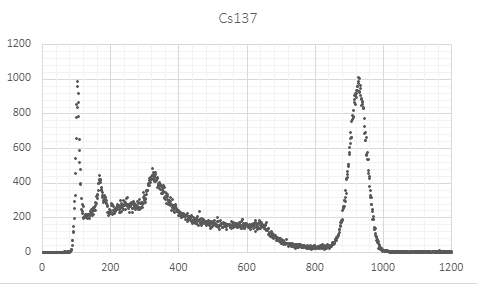
\includegraphics[scale=0.4]{Cs}

Спектр Цезия
\end{center}

У цезия мы наблюдаем один фотопик и выраженную границу Комптон-эффекта.

\subsection*{Натрий, Na}
\begin{center}
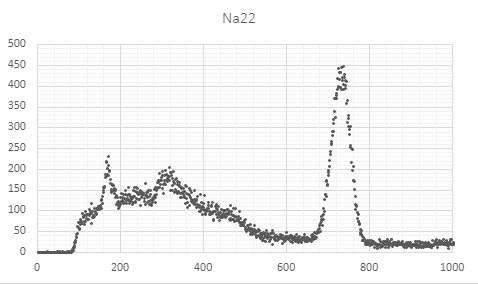
\includegraphics[scale=0.4]{Na}

Спектр Натрия
\end{center}

У натрия мы наблюдаем два фотопика и выраженную границу Комптон-эффекта.

\subsection*{Кобальт, Co}
\begin{center}
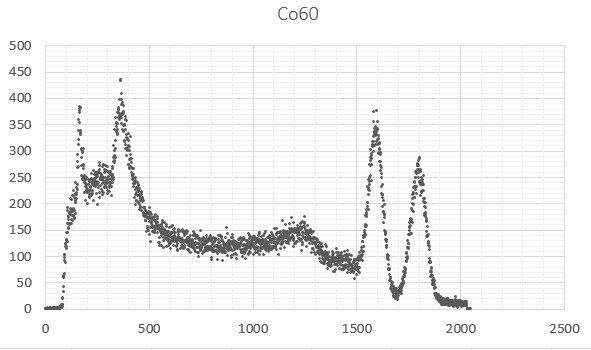
\includegraphics[scale=0.4]{Co}

Спектр Кобальта
\end{center} 

У кобальта два четко выраженных фотопика и выраженная граница Комптон-эффекта.

\subsection*{Америций, Am}
\begin{center}
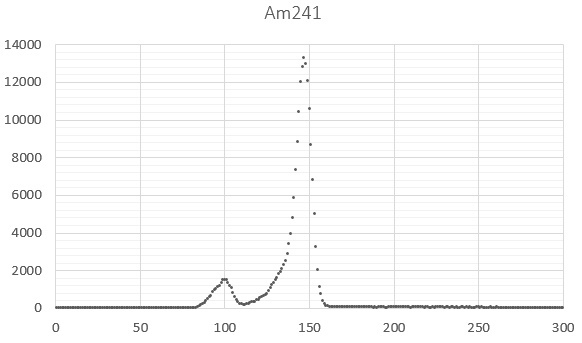
\includegraphics[scale=0.4]{Am}

Спектр Америция
\end{center}

У америция мы наблюдаем один фотопик и неявную границу эффекта Комптона.

\subsection*{Европий, Eu}

\begin{center}
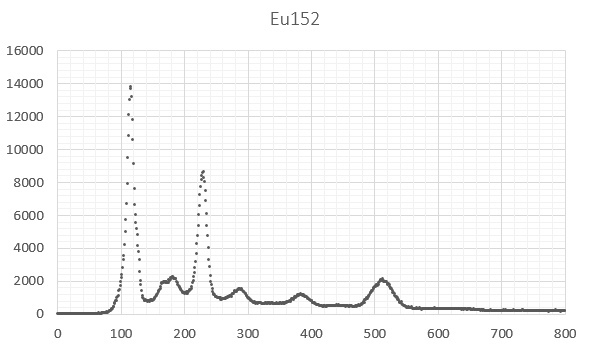
\includegraphics[scale=0.4]{Eu}

Спектр Европия
\end{center}

\section*{Обработка результатов}
В каждом спектре определим номера каналов, отвечающие центрам пиков полного поглощения излучения от радиоактивных источников. Этим каналам присваивают соответствующие табличные значения энергий и проводят линейную аппроксимацию зависимости энергии от номера канала для данного гамма-спектрометра при данной геометрии измерения и настройках гамма-спектрометра. Построим калибровочный график зависимости энергии $\gamma$-кванта от номера канала $N_i$ по данным таблицы 1.
\begin{center}
\includegraphics[scale=0.4]{table1}

Таблица 1.
\end{center}
Уравнение зависимости энергии гамма-квантов от номера канала имеет вид: $E=b\cdot N+a$, где $b=740\pm7\cdot 10^{-6}$, $a=-10\pm 1 \cdot 10^{-3}$.	Нахождение уравнения зависимости проведено методом наименьших квадратов. 

\subsection*{Определение энергии пиков полного поглощения}

Используя калибровочный график, определим для всех остальных источников значение энергии пиков полного поглощения $E_i$, их ширины на половине высоты $\Delta E_i$ и энергетическое разрешение $R_i$. Результаты сведите в таблицу:
\begin{center}
\includegraphics[scale=0.5]{table2}

Таблица 2.
\end{center}
Полученные результаты энергии гамма-квантов для различных источников согласуются с табличными данными в пределах погрешности их определения.

\subsection*{Край комптоновского поглощения}
По результатам измерения энергии края комптоновского поглощения построим составим таблицу экспериментальных и расчётных значений энергии.
\begin{center}
\includegraphics[scale=0.4]{table3}

Таблица 3.
\end{center}

\subsection*{Энергетическое разрешение}
Энергетическое разрешение спектрометра:
\[R_i=\frac{\Delta E_i}{E_i}\]
Значение $E_i$ пропорционально среднему числу фотонов на выходе ФЭУ, т.е:
\[E_i=\alpha \bar{n_i}\]
Полуширина пика полного поглощения пропорциональна среднеквадратичной флуктуации $\bar{\Delta n_i}$. Т. к. $n_i$ является дискретной случайной величиной, которая распределена по закону Пуассона, то
\[\Delta E_i = \alpha \bar{\Delta n_i} = \alpha \sqrt{\bar{n_i}}\]
Получим, что
\begin{equation}
R_i = \frac{\Delta E_i}{E_i} = \frac{const}{\sqrt{E_i}}
\end{equation}

Проверим зависимость (1). Построим по полученным данным таблицы 4 график $R^2_i = f(1/E_i)$. 
\begin{center}
\includegraphics[scale=0.5]{table4}

Таблица 4.
\end{center}
\begin{center}
\includegraphics[scale=0.6]{graph1}

График 1.
\end{center}
Как видно из графика точки ложатся на аппроксимирующую прямую в пределах погрешности.

\section*{Вывод}
Мы определили энергии полного поглощения для разных источников. Полученные данные совпадают с табличными в пределах погрешности их определения. Повысить точность измерения энергии полного поглощения для данных образцом возможно двумя способами: увеличить длительность эксперимента или использовать более сильные источники излучения. Убедились, что число протонов на выходе ФЭУ является дискретной случайной величиной, распределённой по закону Пуассона. С помощью осциллографа пронаблюдали фору импульсов на выходе ФЭУ. 

\end{document} % конец документа
